\chapter{Introducción específica} % Main chapter title

\label{Chapter2}

%----------------------------------------------------------------------------------------
%	SECTION 1
%----------------------------------------------------------------------------------------
Todos los capítulos deben comenzar con un breve párrafo introductorio que indique cuál es el contenido que se encontrará al leerlo.  La redacción sobre el contenido de la memoria debe hacerse en presente y todo lo referido al proyecto en pasado, siempre de modo impersonal.

\section{Componentes principales de hardware}
\label{sec:ejemplo}

\subsection{STM32 NUCLEO-L432KC}
La placa STM32 Nucleo-32 proporciona una forma asequible y flexible para que los usuarios prueben nuevos conceptos y construyan prototipos eligiendo entre las diversas combinaciones de funciones de rendimiento y consumo de energía que proporciona el microcontrolador STM32.
\\Características:
\begin{itemize}
	\item Microcontrolador STM32L4KC en paquete 32 de pines.
	\item 1 led de usuario.
	\item 1 pulsador de reset.
	\item Conector de expasion Arduino Nano V3.
	\item Conector USB Micro-AB para ST-LINK.
	\item Opciones flexibles de funete de alimentacion.
	\item Depurador/Programador ST-LINK integrado.
	\item Comtibilidad con una amplia variedad de entornos de desarrollo integrado.
	\item Oscilador de cristal de 24MHz
	\item Compatible con Arm Mbed Enabled  
  \end{itemize}
\begin{figure}[htbp]
	\centering
	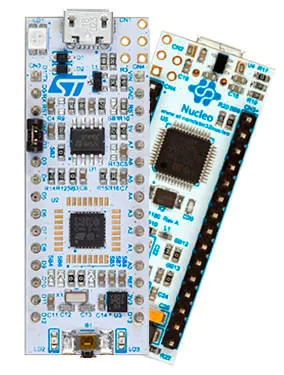
\includegraphics[width=.4\textwidth]{./Figures/nucleo-l432kc.jpg}
	\caption{Modulo LTE IOT 2 CLICK.}
\end{figure}
\vspace{5cm}

\subsection{Modulo Comunicacion LTE IOT 2 CLICK}
\label{subsec:ejemplo}
LTE IoT 2 click está equipado con el módulo BG96 LTE de Quectel Wireless Solutions , que admite tecnologías LTE CAT M1 y NB1, desarrolladas con aplicaciones IoT en mente. Además, admite EGPRS a 850/900/1800/1900 MHz, lo que significa que se puede usar globalmente; no está restringido a ninguna región. El soporte para las tecnologías CAT M1 y NB1 y el consumo de energía ultra bajo hacen de este módulo una elección perfecta para la próxima tecnología 3GPP IoT.
\begin{figure}[htbp]
	\centering
	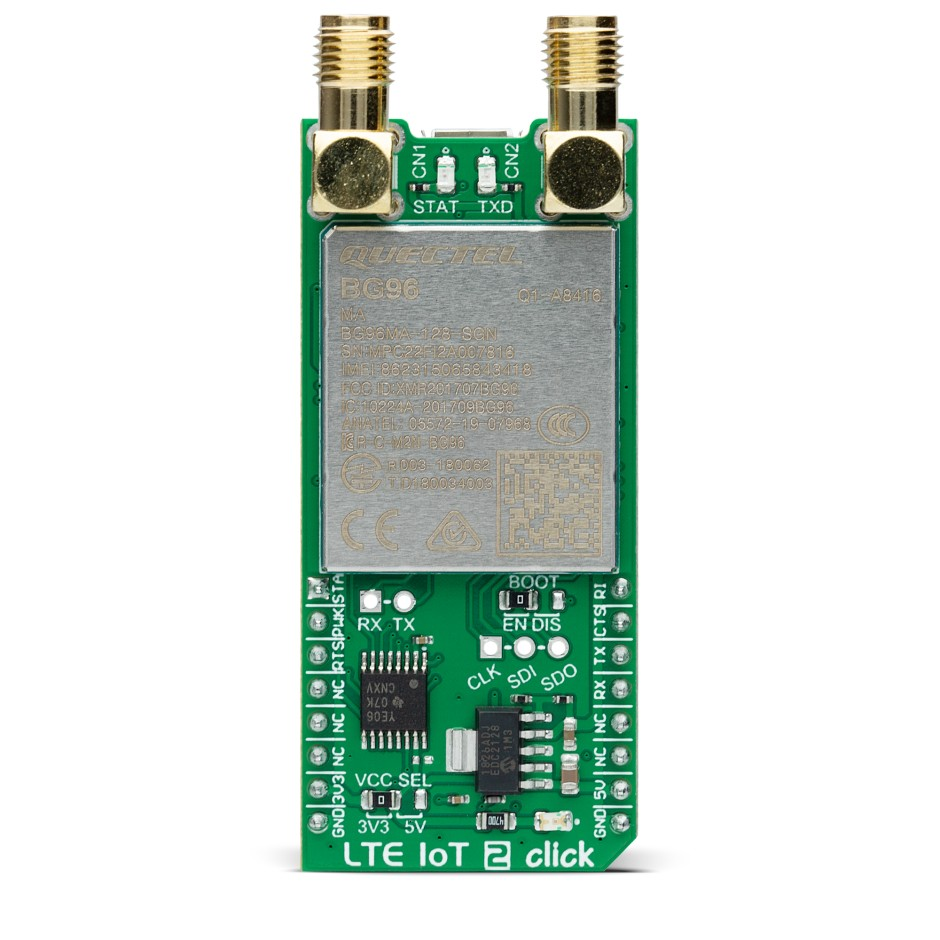
\includegraphics[width=.4\textwidth]{./Figures/moduloBG96.jpg}
	\caption{Modulo LTE IOT 2 CLICK.}
\end{figure}

\subsection{Sensor AHT10}
AHT10 es un sensor que permite obtener lecturas de temperatura y humedad, es de bajo costo y excelente rendimiento. El sensor es muy versátil, puede sustituir a los sensores DHT11, SHT20 y AM2302, debido a su estabilidad en entornos más hostiles. Utiliza este sensor en aplicaciones de control automático de temperatura, aire acondicionado, estaciones meteorológicas, aplicaciones en el hogar, regulador de humedad y temperatura.
\begin{figure}[htbp]
	\centering
	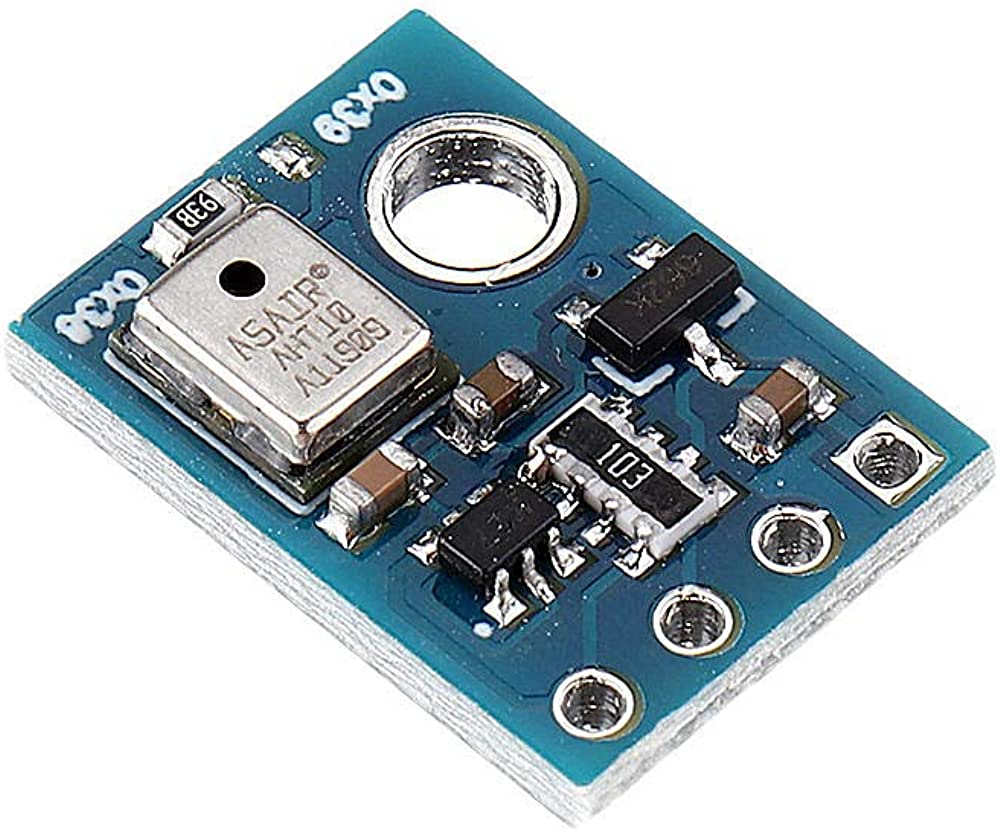
\includegraphics[width=.4\textwidth]{./Figures/aht10.jpg}
	\caption{Modulo LTE IOT 2 CLICK.}
\end{figure}

\subsection{Sensor ML8511}

El módulo ML8511 es un sensor de luz ultravioleta (UV), entrega una señal de voltaje analógica que depende de la cantidad de luz UV que detecta. Sensor ideal para proyectos de monitoreo de condiciones ambientales como el índice UV, Aplicaciones Meteorológicas, cuidado de la piel, medición industrial de nivel UV.
El sensor ML8511 detecta luz con una longitud de onda entre 280-390 nm, este rango cubre tanto al espectro UV-B como al UV-A. La salida analógica está relacionada linealmente con la intensidad UV (mW/cm2). Esta señal analógica puede ser conectada a un microcontrolador para ser convertido por un ADC y así trabajar con la medición. 
\begin{figure}[htbp]
	\centering
	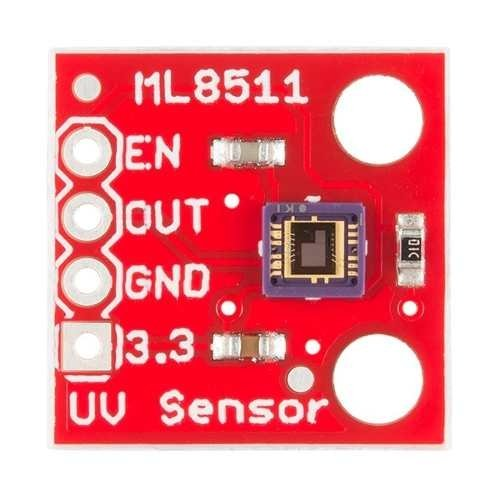
\includegraphics[width=.4\textwidth]{./Figures/ml8511.jpg}
	\caption{Modulo LTE IOT 2 CLICK.}
\end{figure}
\subsection{Sensor de Humedad de Suelo HL-69 (Resistivo)} 
\begin{figure}[htbp]
	\centering
	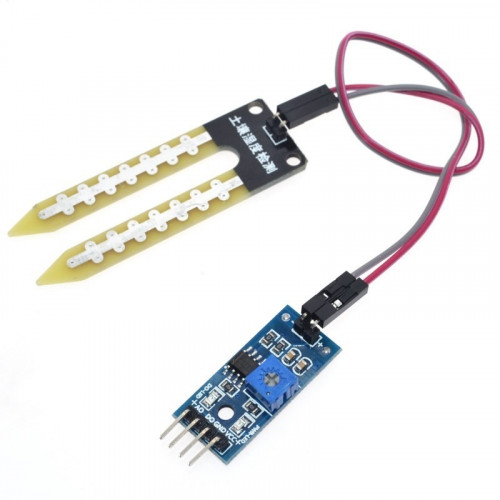
\includegraphics[width=.4\textwidth]{./Figures/sensordehumedad.jpg}
	\caption{Modulo LTE IOT 2 CLICK.}
\end{figure}




Al insertar figuras en la memoria se deben considerar determinadas pautas. Para empezar, usar siempre tipografía claramente legible. Luego, tener claro que \textbf{es incorrecto} escribir por ejemplo esto: ``El diseño elegido es un cuadrado, como se ve en la siguiente figura:''

\begin{figure}[h]
\centering

\includegraphics[scale=.45]{./Figures/cuadradoAzul.png}
\end{figure}

La forma correcta de utilizar una figura es con referencias cruzadas, por ejemplo: ``Se eligió utilizar un cuadrado azul para el logo, como puede observarse en la figura \ref{fig:cuadradoAzul}''.

\begin{figure}[ht]
	\centering
	
\includegraphics[scale=.45]{./Figures/cuadradoAzul.png}
	\caption{Ilustración del cuadrado azul que se eligió para el diseño del logo.}
	\label{fig:cuadradoAzul}
\end{figure}

El texto de las figuras debe estar siempre en español, excepto que se decida reproducir una figura original tomada de alguna referencia. En ese caso la referencia de la cual se tomó la figura debe ser indicada en el epígrafe de la figura e incluida como una nota al pie, como se ilustra en la figura \ref{fig:palabraIngles}.

\begin{figure}[htpb]
	\centering
	
\includegraphics[scale=.3]{./Figures/word.jpeg}
	\caption{Imagen tomada de la página oficial del procesador\protect\footnotemark.}
	\label{fig:palabraIngles}
\end{figure}

\footnotetext{Imagen tomada de \url{https://goo.gl/images/i7C70w}}

La figura y el epígrafe deben conformar una unidad cuyo significado principal pueda ser comprendido por el lector sin necesidad de leer el cuerpo central de la memoria. Para eso es necesario que el epígrafe sea todo lo detallado que corresponda y si en la figura se utilizan abreviaturas entonces aclarar su significado en el epígrafe o en la misma figura.



\begin{figure}[ht]
	\centering
	
\includegraphics[scale=.37]{./Figures/questionMark.png}
	\caption{¿Por qué de pronto aparece esta figura?}
	\label{fig:questionMark}
\end{figure}

Nunca colocar una figura en el documento antes de hacer la primera referencia a ella, como se ilustra con la figura \ref{fig:questionMark}, porque sino el lector no comprenderá por qué de pronto aparece la figura en el documento, lo que distraerá su atención.

Otra posibilidad es utilizar el entorno \textit{subfigure} para incluir más de una figura, como se puede ver en la figura \ref{fig:three graphs}. Notar que se pueden referenciar también las figuras internas individualmente de esta manera: \ref{fig:1de3}, \ref{fig:2de3} y \ref{fig:3de3}.
 
\begin{figure}[!htpb]
     \centering
     \begin{subfigure}[b]{0.3\textwidth}
         \centering
         
\includegraphics[width=.65\textwidth]{./Figures/questionMark}
         \caption{Un caption.}
         \label{fig:1de3}
     \end{subfigure}
     \hfill
     \begin{subfigure}[b]{0.3\textwidth}
         \centering
         
\includegraphics[width=.65\textwidth]{./Figures/questionMark}
         \caption{Otro.}
         \label{fig:2de3}
     \end{subfigure}
     \hfill
     \begin{subfigure}[b]{0.3\textwidth}
         \centering
         
\includegraphics[width=.65\textwidth]{./Figures/questionMark}
         \caption{Y otro más.}
         \label{fig:3de3}
     \end{subfigure}
        \caption{Tres gráficos simples}
        \label{fig:three graphs}
\end{figure}

El código para generar las imágenes se encuentra disponible para su reutilización en el archivo \file{Chapter2.tex}.

\subsection{Tablas}

Para las tablas utilizar el mismo formato que para las figuras, sólo que el epígrafe se debe colocar arriba de la tabla, como se ilustra en la tabla \ref{tab:peces}. Observar que sólo algunas filas van con líneas visibles y notar el uso de las negritas para los encabezados.  La referencia se logra utilizando el comando \verb|\ref{<label>}| donde label debe estar definida dentro del entorno de la tabla.

\begin{verbatim}
\begin{table}[h]
	\centering
	\caption[caption corto]{caption largo más descriptivo}
	\begin{tabular}{l c c}    
		\toprule
		\textbf{Especie}     & \textbf{Tamaño} & \textbf{Valor}\\
		\midrule
		Amphiprion Ocellaris & 10 cm           & \$ 6.000 \\		
		Hepatus Blue Tang    & 15 cm           & \$ 7.000 \\
		Zebrasoma Xanthurus  & 12 cm           & \$ 6.800 \\
		\bottomrule
		\hline
	\end{tabular}
	\label{tab:peces}
\end{table}
\end{verbatim}


\begin{table}[h]
	\centering
	\caption[caption corto]{caption largo más descriptivo}
	\begin{tabular}{l c c}    
		\toprule
		\textbf{Especie} 	 & \textbf{Tamaño} 		& \textbf{Valor}  \\
		\midrule
		Amphiprion Ocellaris & 10 cm 				& \$ 6.000 \\		
		Hepatus Blue Tang	 & 15 cm				& \$ 7.000 \\
		Zebrasoma Xanthurus	 & 12 cm				& \$ 6.800 \\
		\bottomrule
		\hline
	\end{tabular}
	\label{tab:peces}
\end{table}

En cada capítulo se debe reiniciar el número de conteo de las figuras y las tablas, por ejemplo, figura 2.1 o tabla 2.1, pero no se debe reiniciar el conteo en cada sección. Por suerte la plantilla se encarga de esto por nosotros.

\subsection{Ecuaciones}
\label{sec:Ecuaciones}

Al insertar ecuaciones en la memoria dentro de un entorno \textit{equation}, éstas se numeran en forma automática  y se pueden referir al igual que como se hace con las figuras y tablas, por ejemplo ver la ecuación \ref{eq:metric}.

\begin{equation}
	\label{eq:metric}
	ds^2 = c^2 dt^2 \left( \frac{d\sigma^2}{1-k\sigma^2} + \sigma^2\left[ d\theta^2 + \sin^2\theta d\phi^2 \right] \right)
\end{equation}
                                                        
Es importante tener presente que si bien las ecuaciones pueden ser referidas por su número, también es correcto utilizar los dos puntos, como por ejemplo ``la expresión matemática que describe este comportamiento es la siguiente:''

\begin{equation}
	\label{eq:schrodinger}
	\frac{\hbar^2}{2m}\nabla^2\Psi + V(\mathbf{r})\Psi = -i\hbar \frac{\partial\Psi}{\partial t}
\end{equation}

Para generar la ecuación \ref{eq:metric} se utilizó el siguiente código:

\begin{verbatim}
\begin{equation}
	\label{eq:metric}
	ds^2 = c^2 dt^2 \left( \frac{d\sigma^2}{1-k\sigma^2} + 
	\sigma^2\left[ d\theta^2 + 
	\sin^2\theta d\phi^2 \right] \right)
\end{equation}
\end{verbatim}

Y para la ecuación \ref{eq:schrodinger}:

\begin{verbatim}
\begin{equation}
	\label{eq:schrodinger}
	\frac{\hbar^2}{2m}\nabla^2\Psi + V(\mathbf{r})\Psi = 
	-i\hbar \frac{\partial\Psi}{\partial t}
\end{equation}

\end{verbatim}